
\documentclass[UTF8,zihao=-4]{ctexart}
\usepackage[a4paper,top=2.2cm,bottom=2.2cm,left=2.35cm,right=2.35cm]{geometry}
\usepackage{amsmath,amssymb,bm}
\usepackage{graphicx}
\usepackage{float}
\usepackage{booktabs}
\usepackage{array}
\usepackage{longtable}
\usepackage{tabularx}
\usepackage{enumitem}
\usepackage{xcolor}
\usepackage{tcolorbox}
\usepackage{listings}
\usepackage{caption}
\usepackage{fancyhdr}
\usepackage{hyperref}
\hypersetup{colorlinks=true,linkcolor=flightblue,urlcolor=flightorange,citecolor=flightblue}

\definecolor{flightnavy}{HTML}{163A5F}
\definecolor{flightblue}{HTML}{2F7EA8}
\definecolor{flightorange}{HTML}{E58B3A}
\definecolor{flightgreen}{HTML}{4F8A6B}
\definecolor{flightslate}{HTML}{64748B}
\definecolor{flightpaper}{HTML}{F7F9FB}
\definecolor{flightline}{HTML}{D6DEE6}

\setCJKmainfont{Microsoft YaHei}
\setmainfont{Arial}
\setsansfont{Arial}
\setmonofont{Consolas}
\pagestyle{fancy}
\setlength{\headheight}{15pt}
\fancyhf{}
\lhead{\textcolor{flightslate}{FlightResilience 航空网络延误传播与恢复策略}}
\rhead{\textcolor{flightslate}{\thepage}}
\renewcommand{\headrulewidth}{0.3pt}
\captionsetup{font=small,labelfont=bf,labelsep=quad}
\newcommand{\figurenote}[1]{\par\smallskip\noindent\color{flightslate}\footnotesize\textbf{读图：}#1}
\newcommand{\keypoint}[1]{\begin{tcolorbox}[colback=flightpaper,colframe=flightline,boxrule=0.5pt,arc=1.5mm,left=2mm,right=2mm,top=1mm,bottom=1mm]\small #1\end{tcolorbox}}
\lstset{basicstyle=\ttfamily\small,breaklines=true,frame=single,rulecolor=\color{flightline},backgroundcolor=\color{flightpaper},keywordstyle=\color{flightblue},commentstyle=\color{flightslate},stringstyle=\color{flightorange}}
\setlist{itemsep=2pt,topsep=3pt}
\renewcommand{\arraystretch}{1.16}

\title{\bfseries\textcolor{flightnavy}{面向突发扰动的航空网络延误传播识别与恢复策略决策}}
\author{系统工程课程项目 \quad FlightResilience}
\date{数据范围：2024-01-01 至 2024-03-31 \quad 节点：30 个机场 \quad 样本：610,640 条航班记录}

\begin{document}
\maketitle
\begin{abstract}
本文研究航空网络中局部延误如何传播，以及有限恢复资源下如何选择恢复策略。项目使用 U.S. DOT BTS 2024 年 1--3 月航班准点公开数据，样本覆盖 30 个主要机场，共 610,640 条记录、824 条有向航线。技术链路不是单一预测模型，而是将计划阶段延误风险、机场有向网络、ISM 结构解释、状态空间传播仿真和多准则评价连接起来。结果显示：计划阶段最佳模型测试 ROC-AUC 为 0.677，传播矩阵最终谱半径为 0.920；恢复/韧性优先偏好下推荐 动态组合，但风险型决策和成本保守条件下 基准策略 会反超。本文因此给出有条件的管理建议，而不是把某一策略写成无条件最优。
\end{abstract}
\noindent\textbf{关键词：} 航空延误；系统工程；复杂网络；ISM；状态空间；TOPSIS；风险决策；静态 Web Demo

\section{问题背景：从单航班延误到网络恢复}
航空延误常被简化为“某一航班是否晚到”的分类问题，但运行控制面对的是一个网络系统：机场容量、航线连接、飞机和机组轮转、旅客衔接以及外部天气共同作用。一个枢纽机场出现容量下降时，延误不会停在原地；它会沿着航线、前序航班和资源占用关系向外扩散。若研究只停留在预测准确率，仍无法回答恢复管理中更关键的问题：延误将传到哪里，哪些节点应该优先恢复，有限资源应均匀投放还是投向关键位置。

本项目把研究对象定义为航空网络运行系统。系统内部包括机场节点、航线边、计划航班、承运航司、运行状态和恢复资源；系统外部包括天气、高峰需求、空域限制和枢纽容量下降。目标函数也不是单一“延误最小”，而是在运行效率、网络韧性、航班影响、经济性和可实施性之间形成可解释权衡。

\keypoint{课程知识落点：第二章强调整体性、有序相关性、动态性、目标优化和可行性原则。本项目对应地将机场网络作为整体，将航线连接作为有序关系，将扰动传播作为动态过程，将策略评价作为多目标优化，并通过静态 Web Demo 验证可复现与可演示。}

\section{系统工程方法链}
霍尔三维结构为本项目提供了组织框架。逻辑维包含摆明问题、系统设计、方案综合、模型化、最优化、决策和实施计划；时间维对应数据获取、模型训练、仿真评估和部署交付；知识维则综合统计学习、复杂网络、控制论思想、运筹评价和管理决策。切克兰德方法论用于处理目标冲突：乘客、航司、机场和监管者的效用观点并不一致，不能假设存在一个对所有主体都绝对最优的方案。

\begin{align}
p_i &= P(y_i=1\mid x_i)=f(x_i), \quad y_i=\mathbb{1}(\mathrm{ArrDel15})\\
\bm{x}(t+1) &= A\bm{x}(t)+B\bm{u}(t)+G\bm{w}(t)+\bm{\epsilon}(t)\\
C_i &= \frac{D_i^-}{D_i^+ + D_i^-}
\end{align}

式中，$p_i$ 是计划阶段延误概率，$\bm{x}(t)$ 是机场小时延误状态，$A$ 是传播矩阵，$\bm{u}(t)$ 是恢复控制，$C_i$ 是 TOPSIS 接近度。三个公式对应“预测--传播--评价”三层接口，避免模型之间相互脱节。

\section{数据范围、审计与防泄漏}
数据来自 BTS Airline On-Time Performance 月度公开文件。原始三个月文件共 1,658,259 条记录，清洗后按样本内总流量筛选前 30 个机场：ATL、DFW、DEN、ORD、CLT、PHX、LAX、LAS、MCO、LGA 等。这样既保留主要枢纽，又能更完整呈现枢纽之间的网络结构。

\begin{table}[H]\centering\caption{数据资产清单节选}
\begin{tabular}{lrr}
\toprule
数据文件 & 行数 & 列数 \\
\midrule
On\_Time\_Reporting\_Carrier\_On\_Time\_Performance\_1987\_present\_2024\_1.zip & 547271 & 40 \\
On\_Time\_Reporting\_Carrier\_On\_Time\_Performance\_1987\_present\_2024\_2.zip & 519221 & 40 \\
On\_Time\_Reporting\_Carrier\_On\_Time\_Performance\_1987\_present\_2024\_3.zip & 591767 & 40 \\
\bottomrule
\end{tabular}
\end{table}

防泄漏处理是本项目可信度的底线。训练、验证、测试按时间顺序划分；航线历史延误率、机场历史延误率和机场小时历史延误率只由训练窗口估计，再映射到验证和测试窗口；实际起飞、实际到达、实际延误分钟数和延误原因字段不得进入计划阶段模型。

\begin{lstlisting}[language=Python,caption={时间切分与历史风险映射}]
train = df[df["split"] == "train"].copy()
route_rate = train.groupby("route")["ArrDel15"].mean()
origin_rate = train.groupby("Origin")["ArrDel15"].mean()

for part in [train, valid, test]:
    part["route_hist_delay_rate"] = part["route"].map(route_rate).fillna(base_rate)
    part["origin_hist_delay_rate"] = part["Origin"].map(origin_rate).fillna(base_rate)
\end{lstlisting}

\section{探索性分析：延误不是平均噪声}
描述性分析说明，延误具有长尾、时段差异、机场差异、航司差异和航线差异。这个事实决定了恢复资源不能按平均值粗放配置。若将所有机场视作同质节点，模型会低估枢纽和高暴露航线的传播作用。


\begin{figure}[H]
  \centering
  
\includegraphics[width=0.86\linewidth]{../figures/fig_06_delay_distribution.png}
  \caption{到达延误分钟数分布}
  \figurenote{严重延误形成长尾，平均值会被少量极端样本抬高；恢复策略需要压缩尾部而不是只优化均值。}
\end{figure}


\begin{figure}[H]
  \centering
  
\includegraphics[width=0.86\linewidth]{../figures/fig_07_daily_volume_delay.png}
  \caption{每日航班量与延误率趋势}
  \figurenote{航班量和延误率并非同向变化，天气、容量和运行组织会改变同等需求下的系统表现。}
\end{figure}


\begin{figure}[H]
  \centering
  
\includegraphics[width=0.86\linewidth]{../figures/fig_08_week_hour_heatmap.png}
  \caption{星期与计划起飞小时延误率热力图}
  \figurenote{高风险时段集中出现，说明计划小时和历史拥堵变量有实际解释价值。}
\end{figure}


\begin{figure}[H]
  \centering
  
\includegraphics[width=0.86\linewidth]{../figures/fig_09_volume_delay_scatter.png}
  \caption{航班量与延误率散点图}
  \figurenote{高流量机场不必然对应最高延误率，说明恢复优先级需要叠加风险和网络位置。}
\end{figure}


\begin{figure}[H]
  \centering
  
\includegraphics[width=0.86\linewidth]{../figures/fig_10_airport_delay_rank.png}
  \caption{机场延误率排名}
  \figurenote{机场间差异明显，不能把网络看作同质节点集合。}
\end{figure}


\begin{figure}[H]
  \centering
  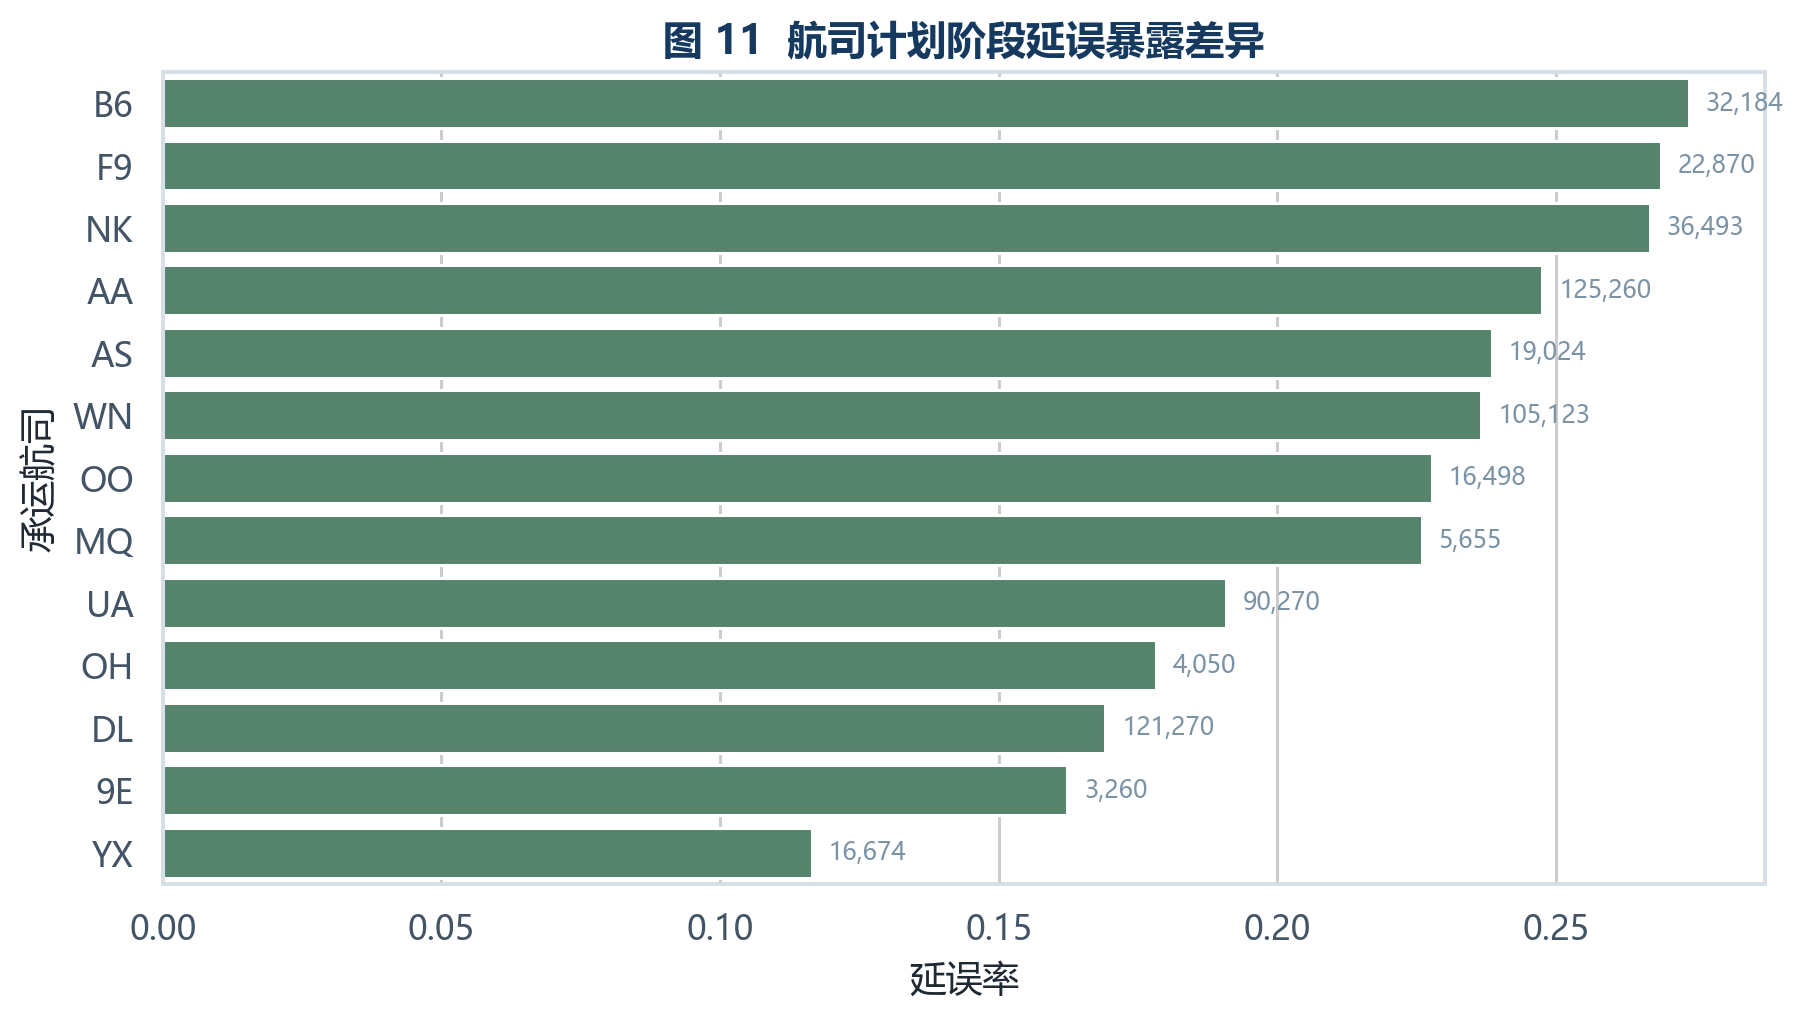
\includegraphics[width=0.86\linewidth]{../figures/fig_11_airline_delay_rank.png}
  \caption{承运航司延误暴露差异}
  \figurenote{航司维度反映机队组织和航线结构差异，是计划阶段风险输入的补充解释。}
\end{figure}


\begin{figure}[H]
  \centering
  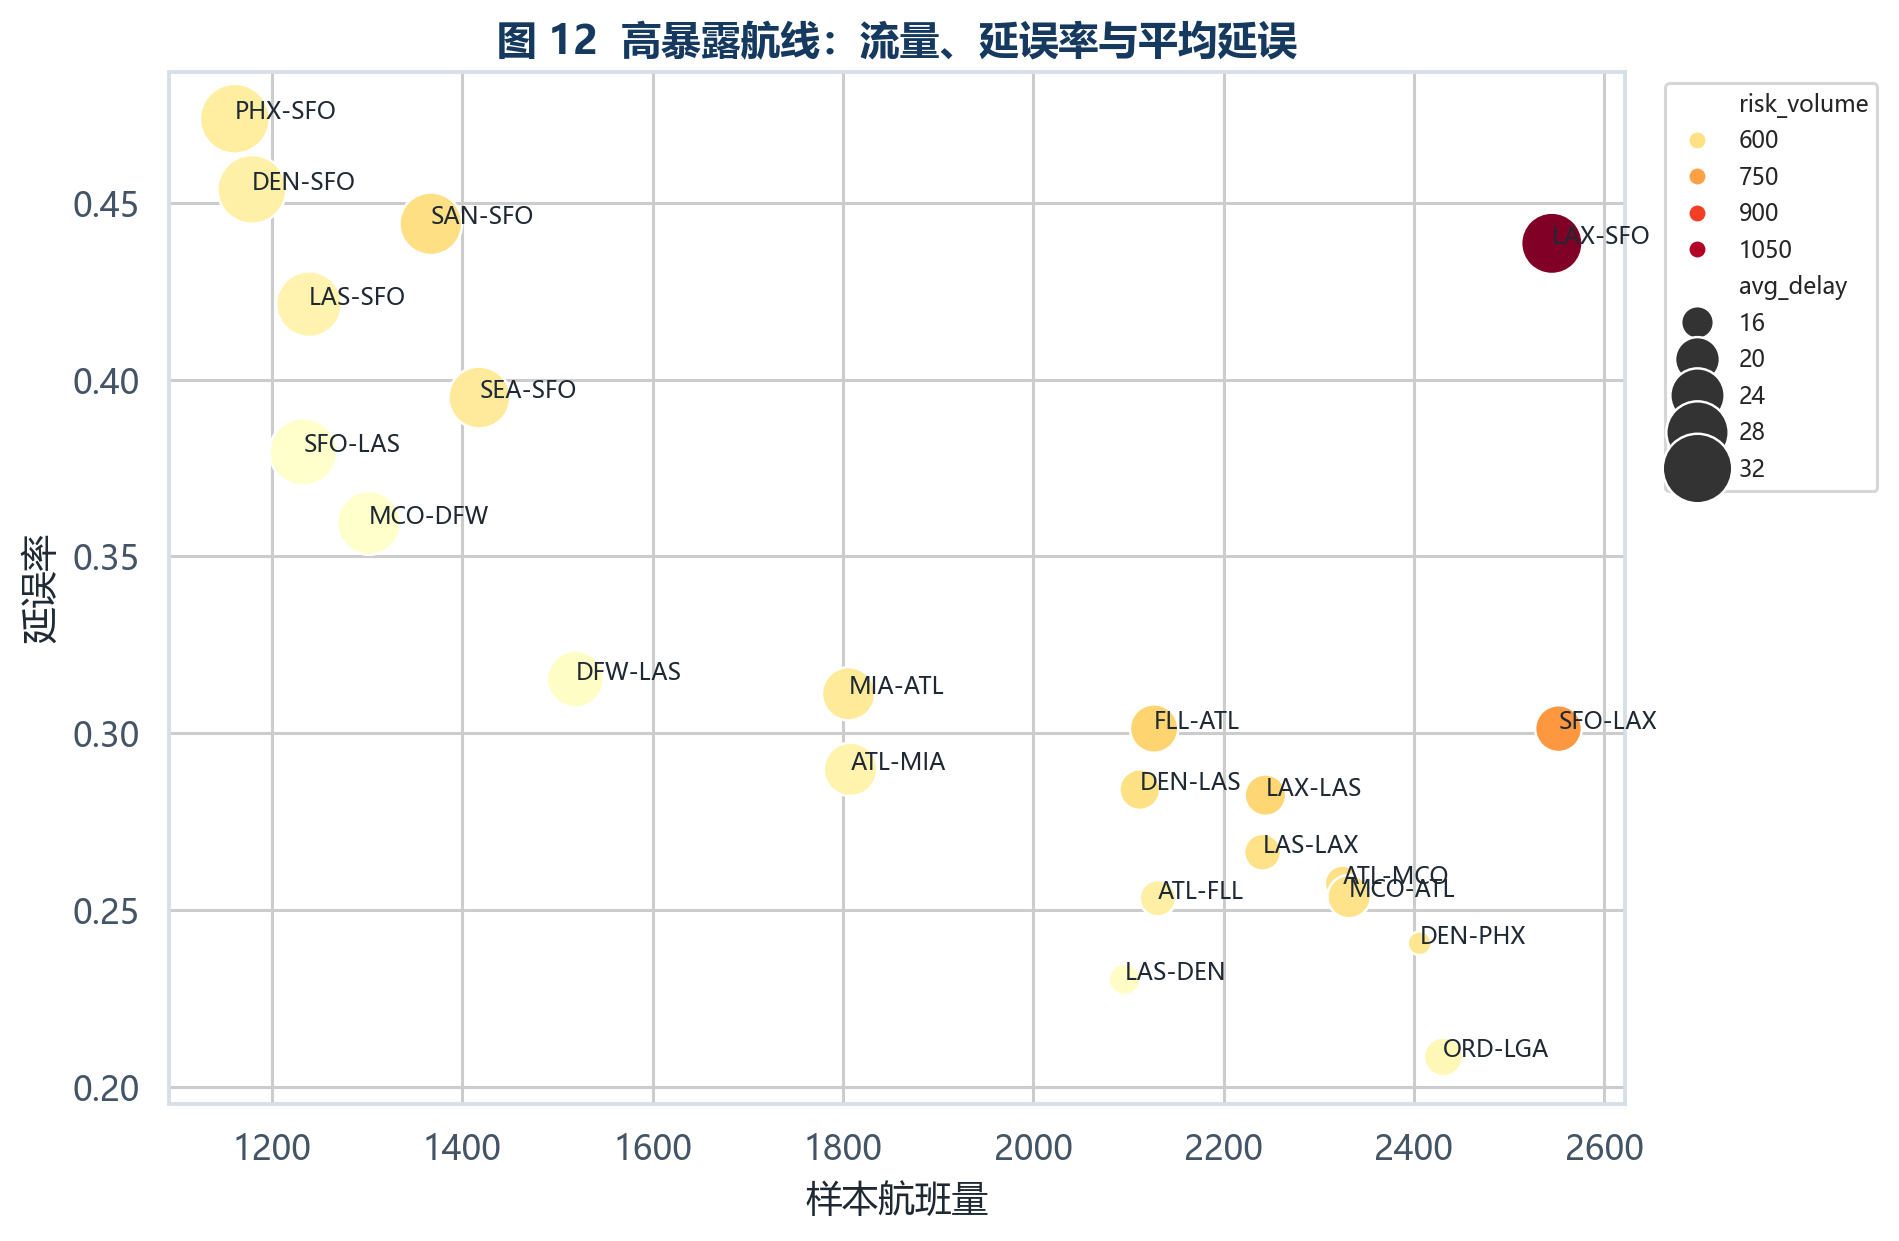
\includegraphics[width=0.86\linewidth]{../figures/fig_12_route_risk_bubble.png}
  \caption{高暴露航线气泡图}
  \figurenote{气泡图同时呈现航班量、延误率和平均延误，帮助识别既高频又高风险的传播通道。}
\end{figure}


\begin{figure}[H]
  \centering
  
\includegraphics[width=0.86\linewidth]{../figures/fig_13_split_delay_rate.png}
  \caption{时间切分目标比例}
  \figurenote{训练、验证、测试目标比例存在差异，说明时间外验证比随机切分更贴近真实部署。}
\end{figure}


\section{计划阶段延误预测}
预测目标为 ArrDel15。本文比较逻辑回归、随机森林和 LightGBM，主模型选择时间外测试表现更稳的 random\_forest。测试 ROC-AUC 为 0.677，PR-AUC 为 0.379。由于延误样本不均衡，PR 曲线比准确率更能说明排序能力。预测模型的定位不是替代调度员，而是为传播矩阵和策略优先级提供风险输入。


\begin{figure}[H]
  \centering
  
\includegraphics[width=0.86\linewidth]{../figures/fig_14_model_metrics.png}
  \caption{时间外测试集模型指标对比}
  \figurenote{随机森林在 ROC-AUC、PR-AUC 和 F1 上较均衡，因此作为后续风险输入模型。}
\end{figure}


\begin{figure}[H]
  \centering
  
\includegraphics[width=0.68\linewidth]{../figures/fig_15_confusion_matrix.png}
  \caption{最佳模型混淆矩阵}
  \figurenote{混淆矩阵用于理解阈值下误报和漏报，策略仿真更关注概率排序与风险输入。}
\end{figure}


\begin{figure}[H]
  \centering
  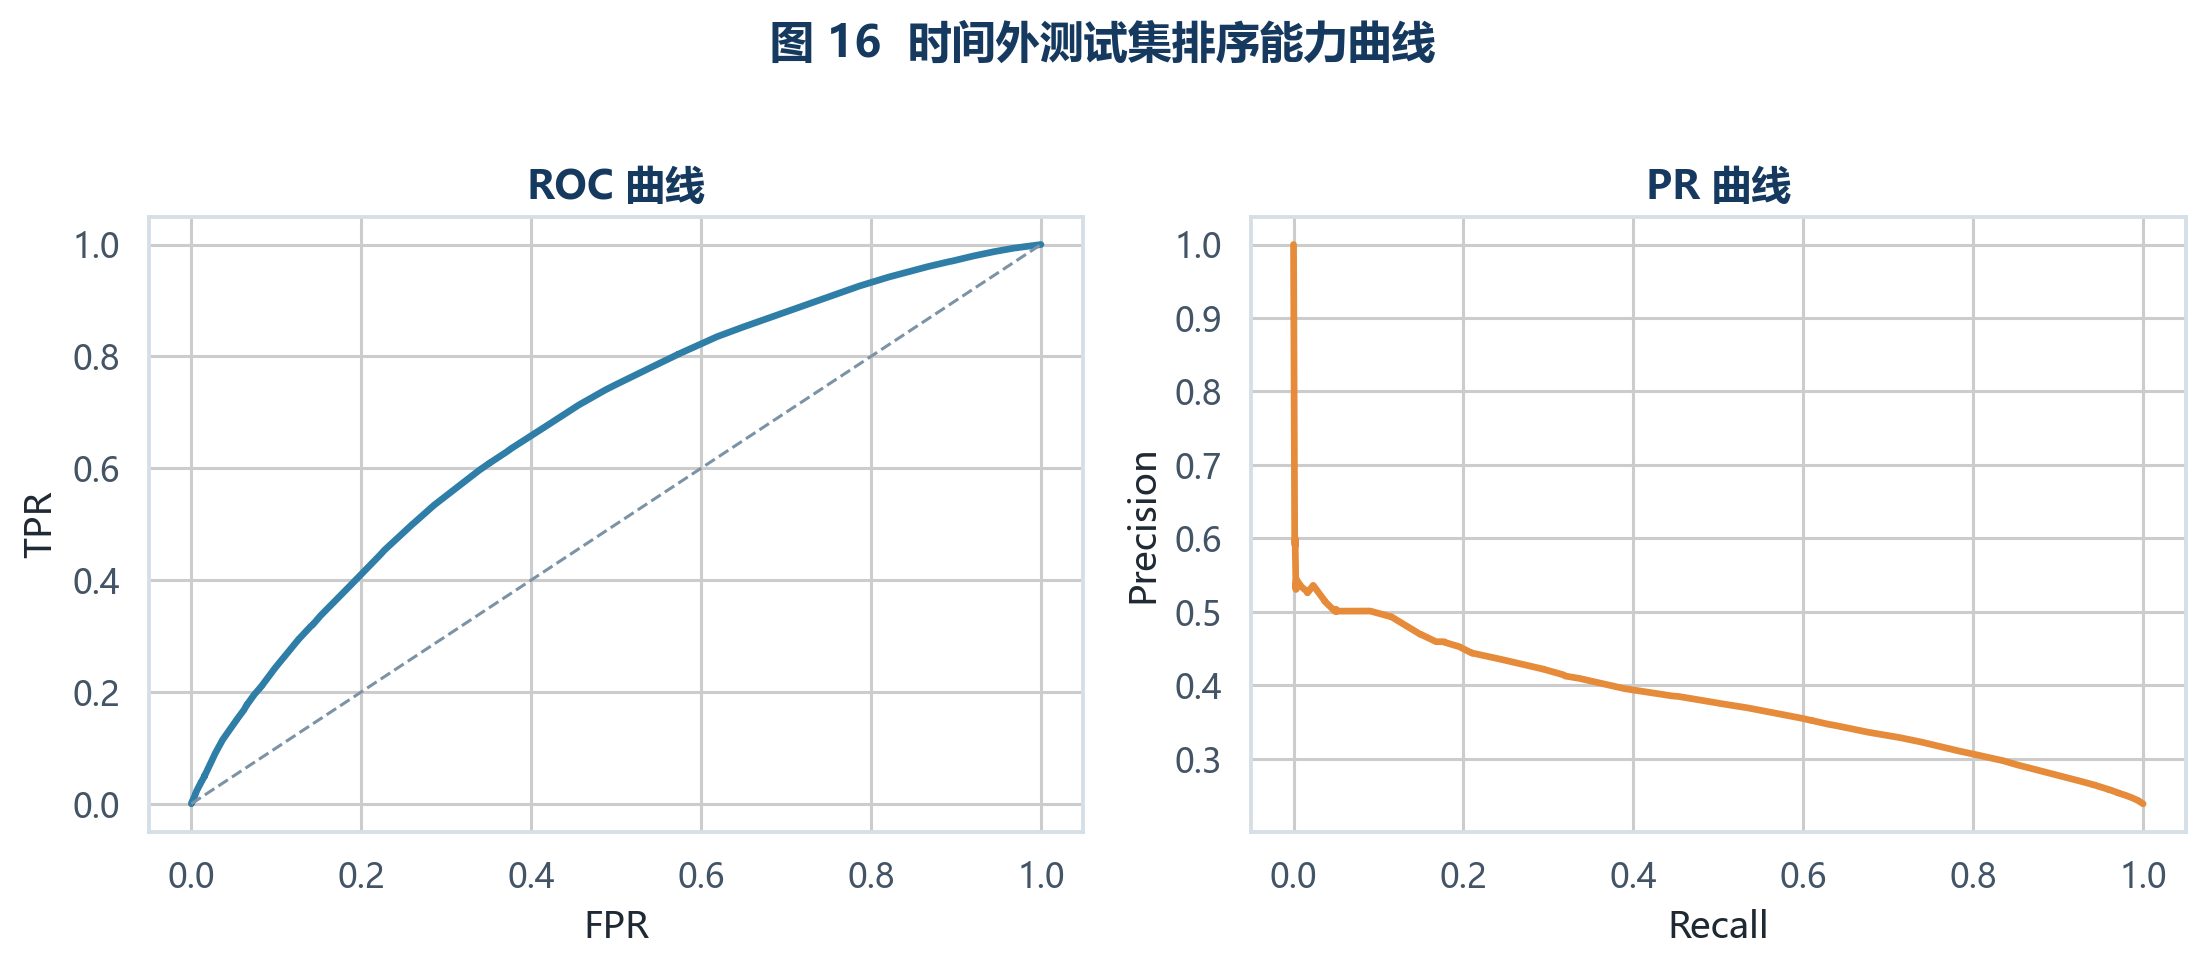
\includegraphics[width=0.86\linewidth]{../figures/fig_16_roc_pr_curves.png}
  \caption{时间外测试集 ROC 与 PR 曲线}
  \figurenote{PR 曲线比准确率更适合延误这种非均衡问题；模型用于排序和风险输入，而不是独立给出最终调度命令。}
\end{figure}


\begin{figure}[H]
  \centering
  
\includegraphics[width=0.68\linewidth]{../figures/fig_17_calibration_curve.png}
  \caption{概率校准曲线}
  \figurenote{概率若严重失真，会影响动态组合策略的风险权重；校准图用于检查概率输出是否可解释。}
\end{figure}


\begin{figure}[H]
  \centering
  
\includegraphics[width=0.86\linewidth]{../figures/fig_18_shap_summary.png}
  \caption{SHAP 全局特征重要性}
  \figurenote{历史延误、机场小时特征和航线经验风险较重要，说明计划阶段信息仍能形成可解释风险估计。}
\end{figure}


\section{机场网络与关键节点}
以机场为节点、航线为有向边后，网络共有 30 个节点、824 条边，最大强连通分量包含全部节点。综合关键性指标为：
\begin{equation}
K_i = 0.25\,\widetilde{flow_i}+0.25\,\widetilde{betweenness_i}+0.25\,\widetilde{risk_i}+0.25\,\widetilde{delay_i}
\end{equation}
当前样本下关键节点前列为：MIA、DEN、DFW、FLL、MCO。这说明扩展样本后默认冲击节点从原先的 DEN 转向 MIA，模型结论随数据范围更新，而不是固定背诵一个机场。

\begin{table}[H]\centering\caption{关键机场指标节选}
\begin{tabular}{lrrrrrr}
\toprule
机场 & 出港 & 到港 & 延误率 & 预测风险 & PageRank & 关键性 \\
\midrule
MIA & 21179 & 21175 & 0.313 & 0.306 & 0.035 & 0.860 \\
DEN & 31253 & 31235 & 0.252 & 0.280 & 0.050 & 0.823 \\
DFW & 27582 & 27537 & 0.273 & 0.278 & 0.044 & 0.758 \\
FLL & 18125 & 18122 & 0.303 & 0.272 & 0.031 & 0.758 \\
MCO & 27400 & 27424 & 0.261 & 0.229 & 0.044 & 0.706 \\
CLT & 21418 & 21434 & 0.238 & 0.245 & 0.035 & 0.647 \\
LAS & 24678 & 24598 & 0.228 & 0.233 & 0.040 & 0.642 \\
ORD & 30678 & 30670 & 0.217 & 0.221 & 0.049 & 0.627 \\
LAX & 29092 & 29116 & 0.209 & 0.203 & 0.046 & 0.603 \\
ATL & 34569 & 34577 & 0.196 & 0.178 & 0.055 & 0.592 \\
SFO & 19362 & 19313 & 0.257 & 0.229 & 0.032 & 0.539 \\
PHX & 25069 & 25041 & 0.197 & 0.200 & 0.041 & 0.538 \\
\bottomrule
\end{tabular}
\end{table}


\begin{figure}[H]
  \centering
  
\includegraphics[width=0.92\linewidth]{../figures/fig_20_airport_network.png}
  \caption{30 节点机场有向航线网络}
  \figurenote{扩展到 30 个机场后，网络更接近真实枢纽结构；标注保留关键节点以避免视觉拥挤。}
\end{figure}


\begin{figure}[H]
  \centering
  
\includegraphics[width=0.86\linewidth]{../figures/fig_21_airport_criticality.png}
  \caption{关键机场综合风险指数排名}
  \figurenote{综合关键性把流量、中心性、预测风险和历史延误合成同一管理指标。}
\end{figure}


\begin{figure}[H]
  \centering
  
\includegraphics[width=0.86\linewidth]{../figures/fig_22_network_risk_scatter.png}
  \caption{中心性、风险与航班量关系}
  \figurenote{同一节点可能高中心但风险中等，或高风险但中心性一般，这正是网络决策需要区别对待的地方。}
\end{figure}


\begin{figure}[H]
  \centering
  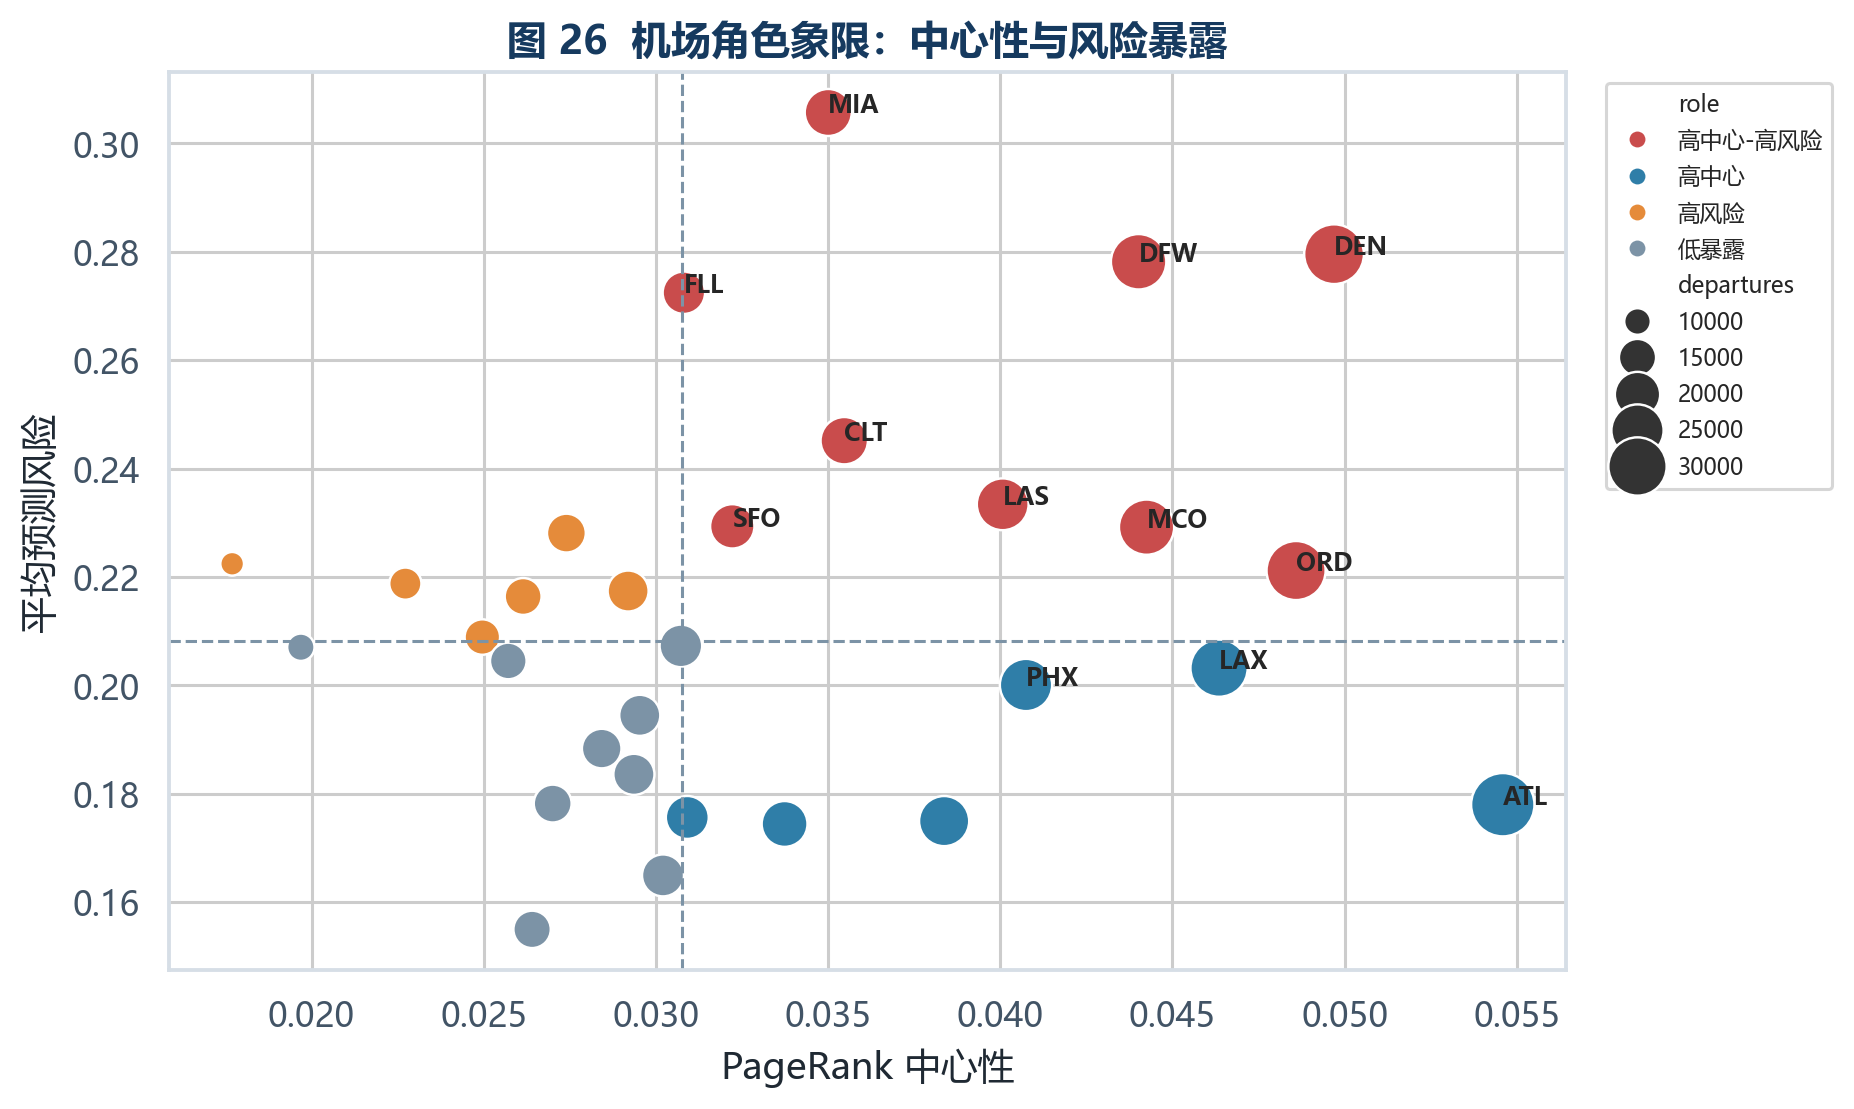
\includegraphics[width=0.86\linewidth]{../figures/fig_26_airport_role_quadrant.png}
  \caption{机场角色象限：中心性与风险暴露}
  \figurenote{高中心高风险机场更适合作为动态组合策略的优先候选，低中心高风险机场则更像局部运行问题。}
\end{figure}


\section{ISM 结构解释}
ISM 结构把天气、容量、计划缓冲、前序晚到、机场拥堵、跨机场传播和恢复时间联系起来。它不是严格因果证明，而是系统结构解释工具：底层因素触发局部运行压力，中间层通过拥堵和前序晚到传导，上层表现为传播范围扩大和恢复时间增加。这一层解释弥补了机器学习特征重要性只描述相关性的不足。


\begin{figure}[H]
  \centering
  
\includegraphics[width=0.86\linewidth]{../figures/fig_25_ism_hierarchy.png}
  \caption{延误因素多级递阶结构}
  \figurenote{ISM 将根源因素、传导因素和结果层分开，使报告能够解释“为什么要做传播仿真”。}
\end{figure}


\begin{figure}[H]
  \centering
  
\includegraphics[width=0.72\linewidth]{../figures/fig_23_ism_adjacency.png}
  \caption{ISM 邻接矩阵}
  \figurenote{邻接矩阵表达直接影响关系，是可达矩阵和层级划分的基础。}
\end{figure}


\begin{figure}[H]
  \centering
  
\includegraphics[width=0.72\linewidth]{../figures/fig_24_ism_reachability.png}
  \caption{ISM 可达矩阵}
  \figurenote{可达矩阵表达直接和间接关系，帮助识别上游驱动因素与表层结果。}
\end{figure}


\section{状态传播仿真}
机场小时平均正延误作为状态变量，传播矩阵 $A$ 由带网络掩码的 Ridge 滞后回归估计。若某机场之间没有航线连接，则不允许其直接进入对方的滞后解释变量，避免无意义全连接。估计后单步 MAE 为 9.74 分钟，最终谱半径为 0.920。

\begin{lstlisting}[language=Python,caption={带网络掩码估计传播矩阵}]
for dest in airports:
    allowed = [origin for origin in airports if origin == dest or (origin, dest) in edge_set]
    model = Ridge(alpha=12.0)
    model.fit(X_lag[:, allowed], y_next[:, dest_index])
    A[dest_index, allowed] = np.maximum(model.coef_, 0)
\end{lstlisting}


\begin{figure}[H]
  \centering
  
\includegraphics[width=0.86\linewidth]{../figures/fig_27_propagation_matrix.png}
  \caption{状态传播矩阵 A}
  \figurenote{矩阵反映延误状态在机场间的滞后传播强度，谱半径约束保证仿真稳定。}
\end{figure}


\begin{figure}[H]
  \centering
  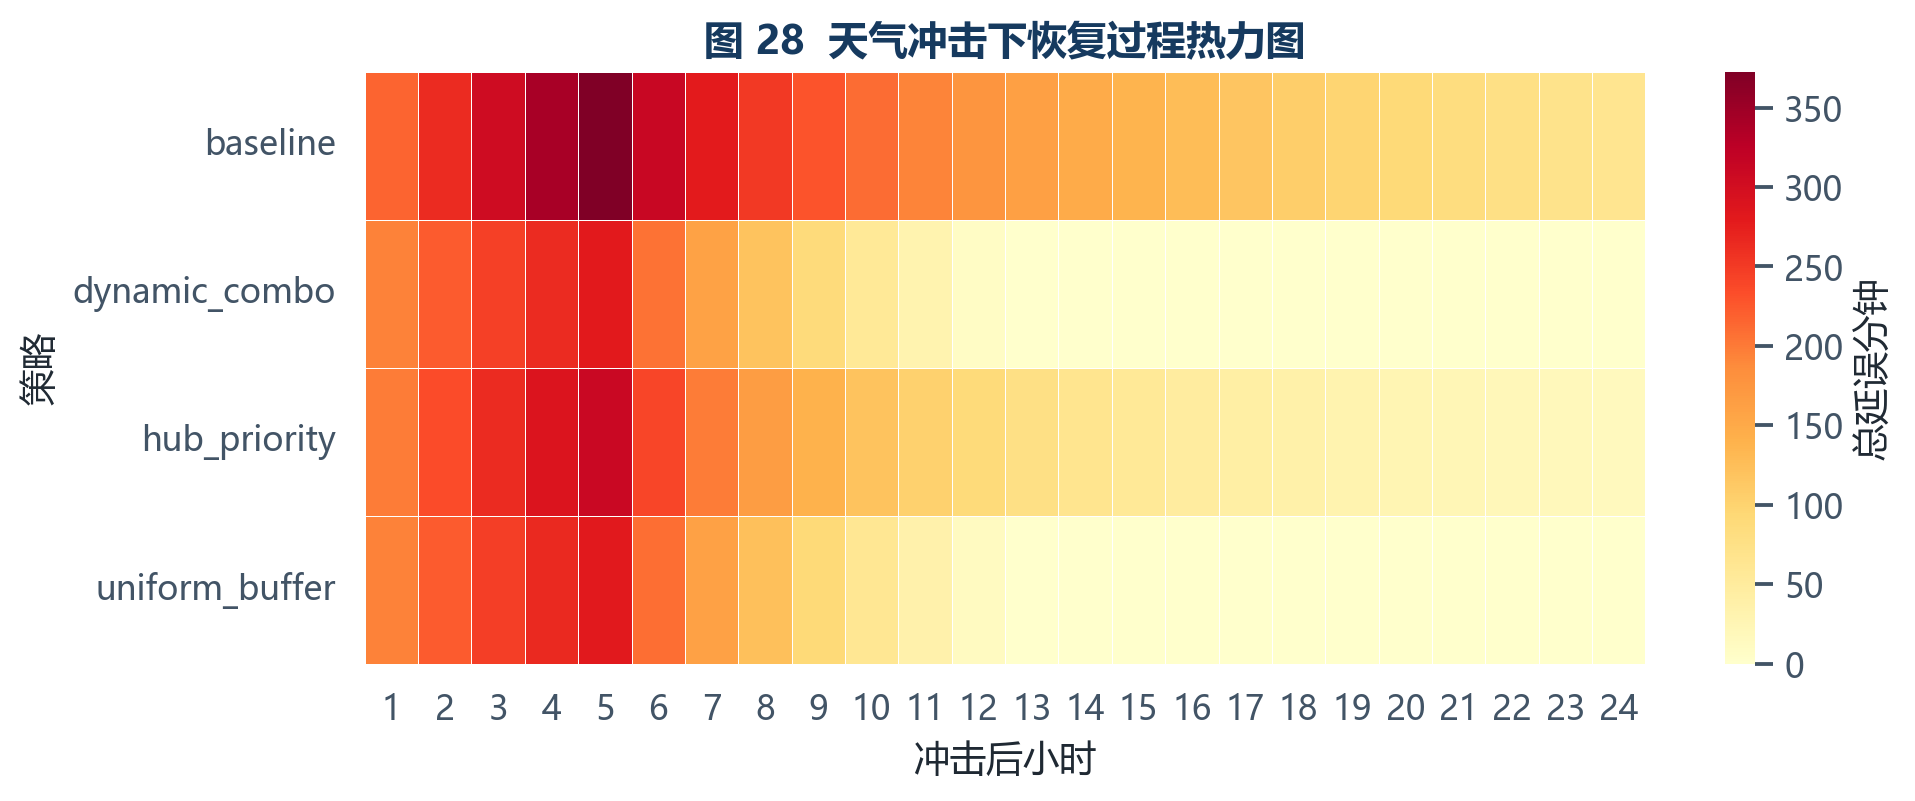
\includegraphics[width=0.86\linewidth]{../figures/fig_28_recovery_heatmap.png}
  \caption{天气冲击下恢复过程热力图}
  \figurenote{热力图显示不同策略在同一冲击下的衰减速度，动态组合较快压低总延误。}
\end{figure}


\begin{figure}[H]
  \centering
  
\includegraphics[width=0.86\linewidth]{../figures/fig_29_recovery_curves.png}
  \caption{天气冲击下系统性能恢复曲线}
  \figurenote{曲线直接比较四类策略的恢复速度和最低性能。}
\end{figure}


\begin{figure}[H]
  \centering
  
\includegraphics[width=0.86\linewidth]{../figures/fig_30_scenario_delay_compare.png}
  \caption{多情景累计延误对比}
  \figurenote{不同情景下策略表现并不完全相同，压力测试可以避免只在单一场景下得出结论。}
\end{figure}


\begin{figure}[H]
  \centering
  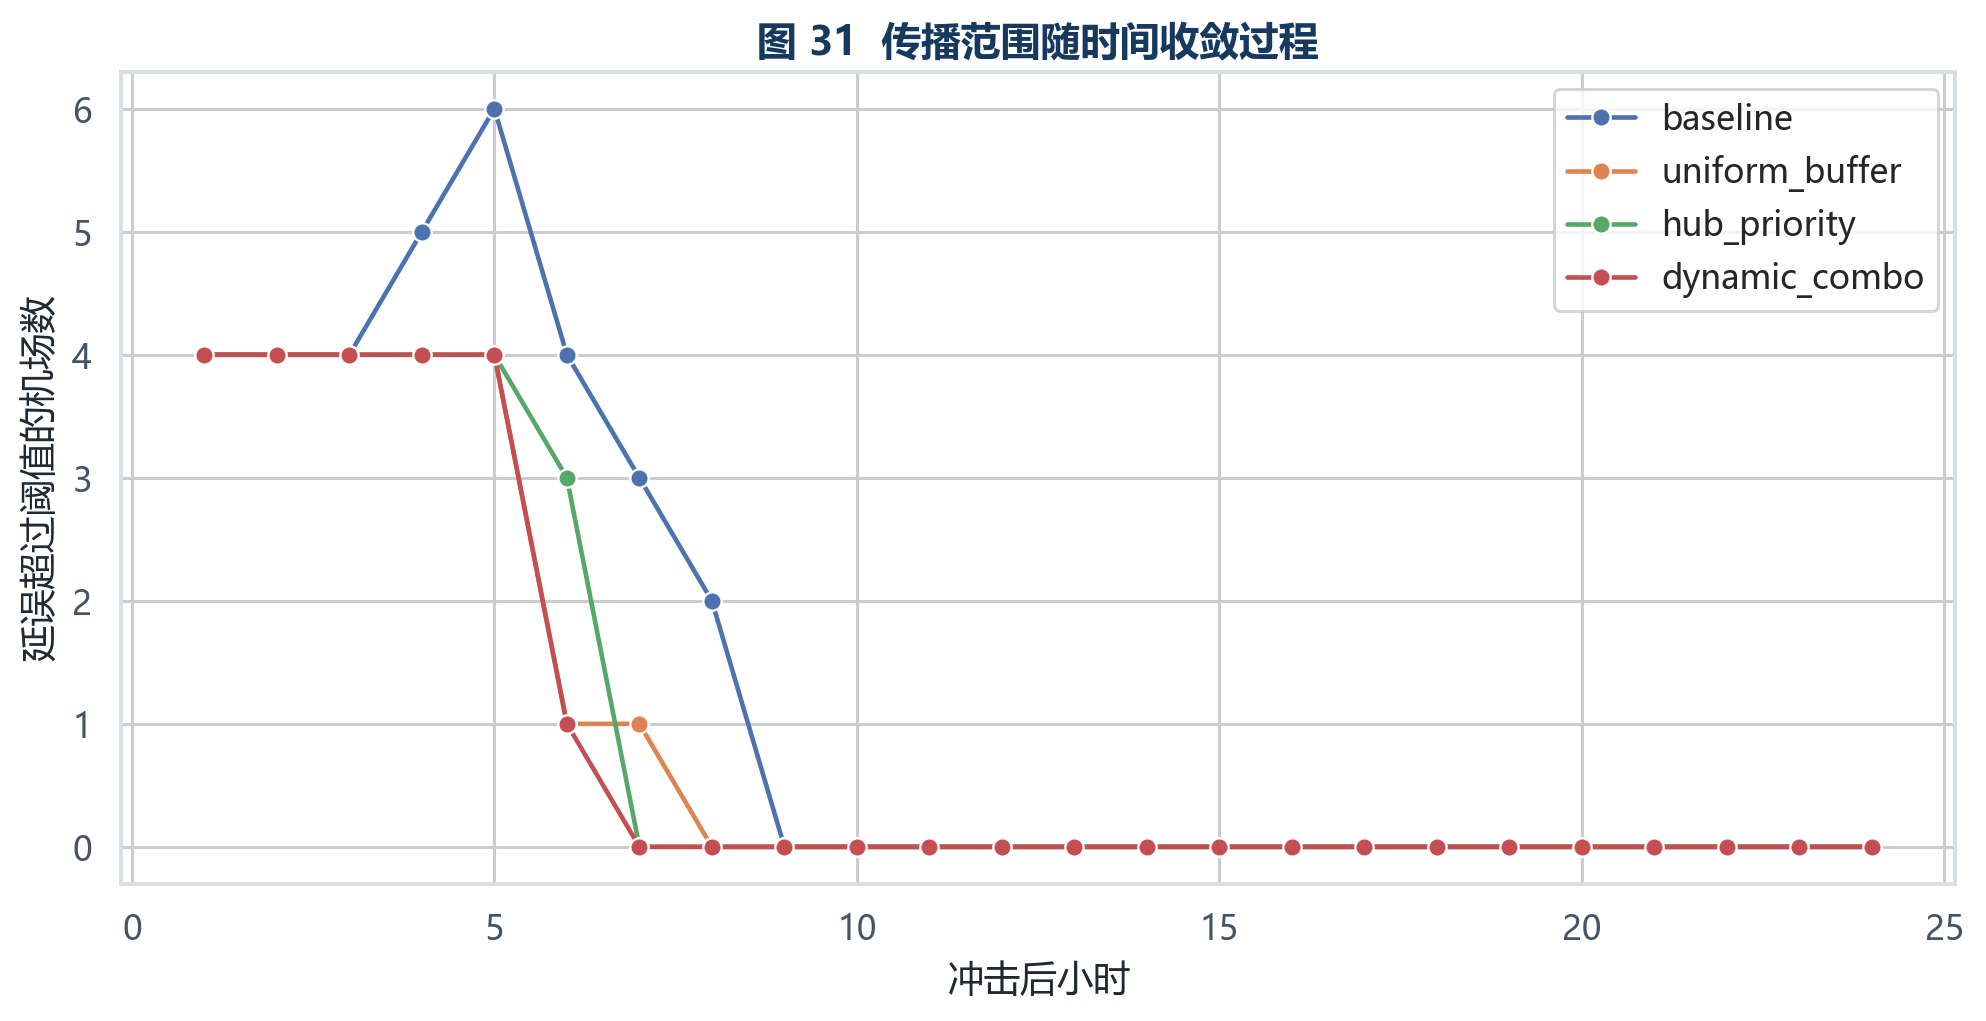
\includegraphics[width=0.86\linewidth]{../figures/fig_31_spread_range_curves.png}
  \caption{传播范围随时间收敛过程}
  \figurenote{传播范围指标避免只看总延误，可反映扰动是否在网络中持续扩散。}
\end{figure}


\begin{figure}[H]
  \centering
  
\includegraphics[width=0.86\linewidth]{../figures/fig_32_cost_delay_pareto.png}
  \caption{成本-延误 Pareto 关系}
  \figurenote{策略选择不是只看恢复效果，也要看资源成本是否过高。}
\end{figure}


\begin{figure}[H]
  \centering
  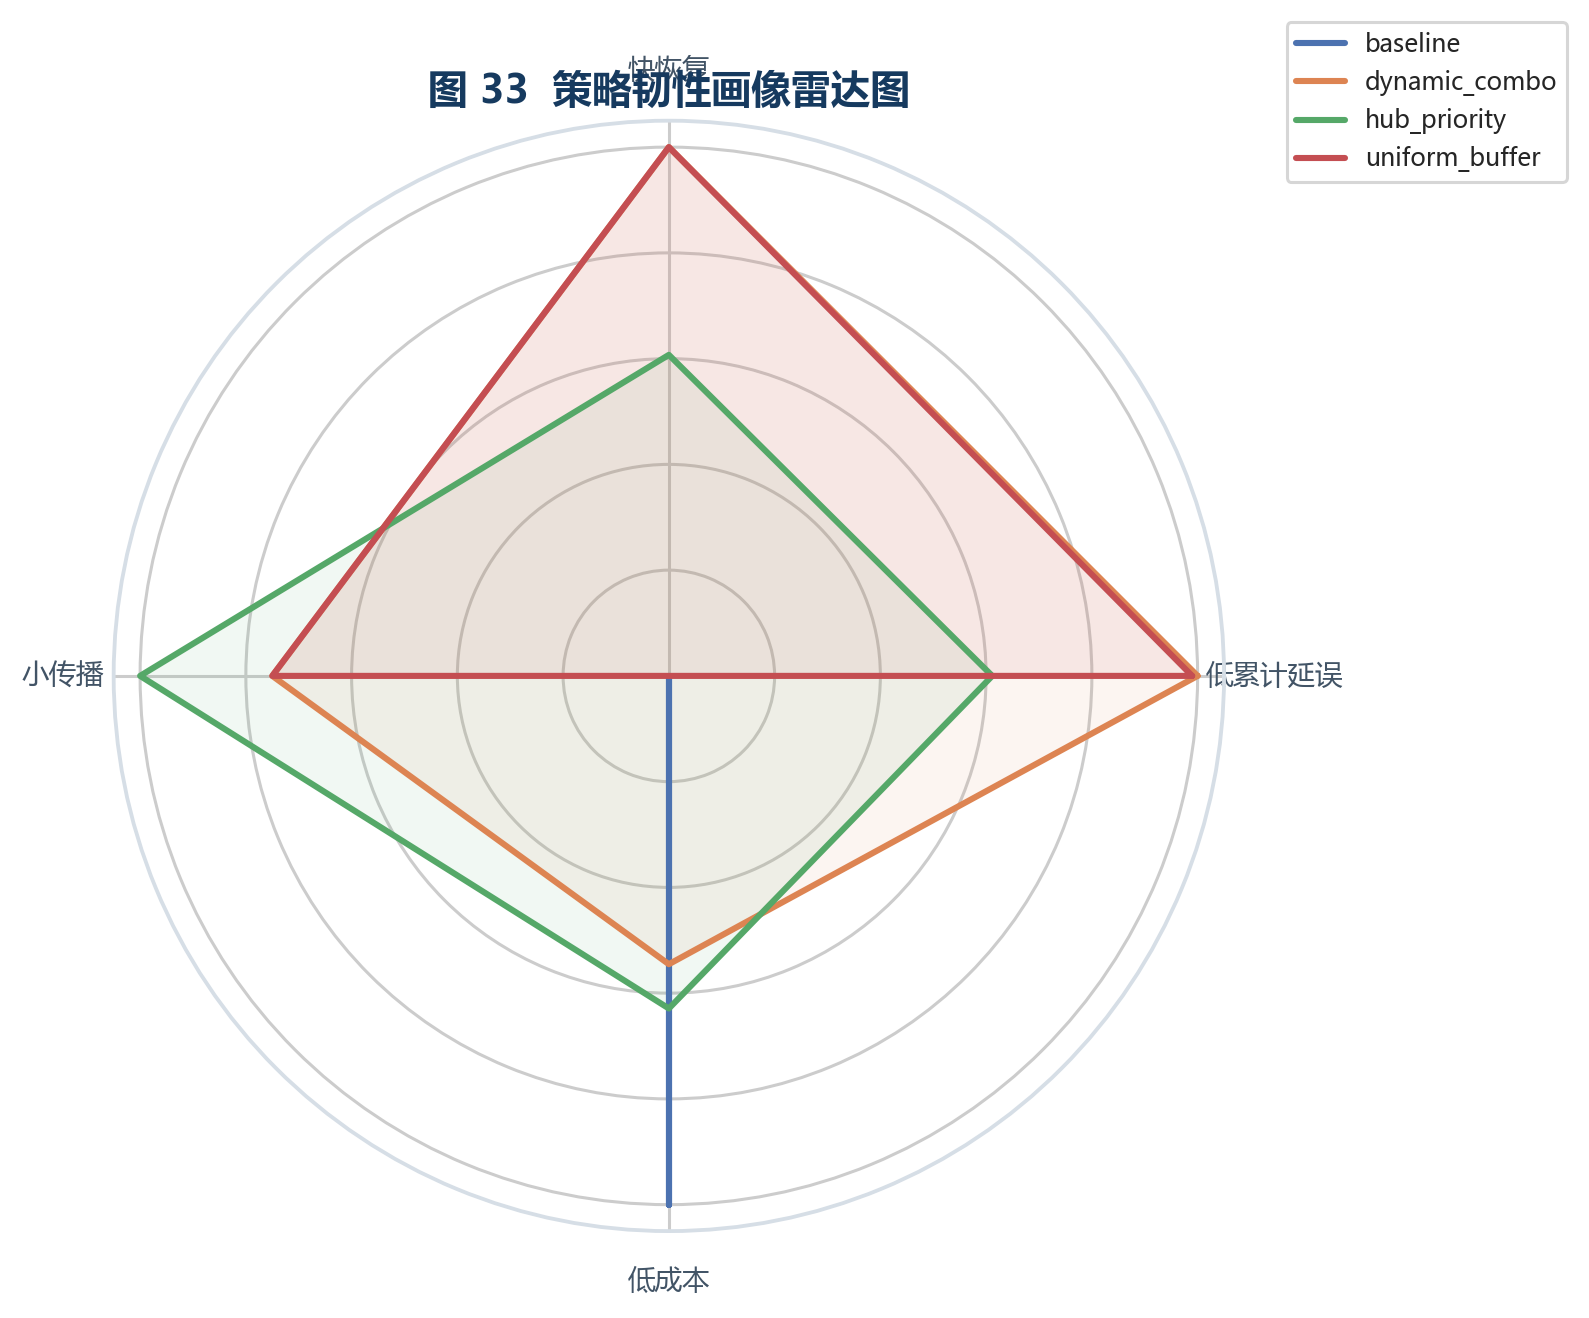
\includegraphics[width=0.70\linewidth]{../figures/fig_33_strategy_radar.png}
  \caption{策略韧性画像雷达图}
  \figurenote{雷达图用于比较低延误、快恢复、小传播和低成本四类目标的折中。}
\end{figure}


\section{多准则评价与风险决策}
策略集合包括基准运行、统一缓冲、关键枢纽优先和动态组合。评价指标覆盖累计延误、平均延误、恢复时间、最低性能、损失面积、传播范围、延误航班比例、取消代理、相对成本和策略复杂度。成本型指标先正向化，再组合 AHP 与熵权。

\begin{equation}
e_j=-k\sum_i p_{ij}\ln p_{ij}, \qquad
w_j=\frac{1-e_j}{\sum_j(1-e_j)}, \qquad
E(L_s)=\sum_c P(c)L_{s,c}
\end{equation}

\begin{table}[H]\centering\caption{主偏好下策略综合排名}
\begin{tabular}{lrrrrr}
\toprule
策略 & TOPSIS & 累计延误 & 恢复时间 & 最低性能 & 成本 \\
\midrule
dynamic\_combo & 0.674 & 976.764 & 7.500 & 0.784 & 730.752 \\
uniform\_buffer & 0.665 & 996.032 & 7.500 & 0.783 & 1,607 \\
hub\_priority & 0.613 & 1,704 & 13.000 & 0.763 & 596.160 \\
baseline & 0.502 & 2,849 & 21.500 & 0.715 & 0.000 \\
\bottomrule
\end{tabular}
\end{table}

\begin{table}[H]\centering\caption{指标权重结构}
\begin{tabular}{lrrrr}
\toprule
指标 & 准则层 & AHP & 熵权 & 组合权重 \\
\midrule
累计总延误 & 运行效率 & 0.148 & 0.066 & 0.140 \\
恢复时间 & 运行效率 & 0.130 & 0.117 & 0.128 \\
最低性能 & 网络韧性 & 0.130 & 0.084 & 0.125 \\
平均延误 & 运行效率 & 0.111 & 0.066 & 0.107 \\
恢复损失面积 & 网络韧性 & 0.111 & 0.066 & 0.107 \\
传播范围 & 网络韧性 & 0.093 & 0.066 & 0.090 \\
延误航班比例 & 航班影响 & 0.093 & 0.066 & 0.090 \\
相对策略成本 & 经济性 & 0.074 & 0.192 & 0.086 \\
策略复杂度 & 可实施性 & 0.056 & 0.222 & 0.072 \\
取消代理数量 & 航班影响 & 0.056 & 0.056 & 0.056 \\
\bottomrule
\end{tabular}
\end{table}

\begin{table}[H]\centering\caption{风险型决策期望损失}
\begin{tabular}{lrr}
\toprule
策略 & 期望损失 & 排名 \\
\midrule
baseline & 1,309 & 1 \\
dynamic\_combo & 1,922 & 2 \\
hub\_priority & 1,957 & 3 \\
uniform\_buffer & 3,680 & 4 \\
\bottomrule
\end{tabular}
\end{table}

\begin{table}[H]\centering\caption{多情景策略表现长表}
\begin{tabular}{lrrrrr}
\toprule
情景 & 策略 & 累计延误 & 恢复时间 & 最低性能 & 成本 \\
\midrule
normal & baseline & 1,544 & 16 & 0.836 & 0.000 \\
normal & uniform\_buffer & 331.211 & 4 & 0.862 & 1,607 \\
normal & hub\_priority & 836.935 & 8 & 0.858 & 596.160 \\
normal & dynamic\_combo & 323.293 & 4 & 0.862 & 730.752 \\
peak & baseline & 2,081 & 20 & 0.790 & 0.000 \\
peak & uniform\_buffer & 550.665 & 6 & 0.844 & 1,607 \\
peak & hub\_priority & 1,159 & 11 & 0.834 & 596.160 \\
peak & dynamic\_combo & 536.607 & 6 & 0.844 & 730.752 \\
weather & baseline & 4,438 & 25 & 0.562 & 0.000 \\
weather & uniform\_buffer & 1,906 & 11 & 0.668 & 1,607 \\
weather & hub\_priority & 2,820 & 18 & 0.634 & 596.160 \\
weather & dynamic\_combo & 1,877 & 11 & 0.670 & 730.752 \\
hub\_failure & baseline & 3,332 & 25 & 0.670 & 0.000 \\
hub\_failure & uniform\_buffer & 1,196 & 9 & 0.758 & 1,607 \\
hub\_failure & hub\_priority & 1,999 & 15 & 0.728 & 596.160 \\
hub\_failure & dynamic\_combo & 1,170 & 9 & 0.761 & 730.752 \\
\bottomrule
\end{tabular}
\end{table}

主偏好下 动态组合 排名第一，主要因为它利用预测风险、关键性、当前状态和下游传播能力动态分配恢复资源。但风险型决策推荐 基准策略，说明成本保守或损失规避的管理者可能做出不同选择。这个分歧不是模型失败，而是系统工程决策中评价主体和价值准则不同的正常结果。


\begin{figure}[H]
  \centering
  
\includegraphics[width=0.86\linewidth]{../figures/fig_34_topsis_score.png}
  \caption{主偏好下 TOPSIS 接近度}
  \figurenote{dynamic\_combo 在主偏好下得分最高，但领先幅度需要结合敏感性分析解释。}
\end{figure}


\begin{figure}[H]
  \centering
  
\includegraphics[width=0.86\linewidth]{../figures/fig_35_fuzzy_grades.png}
  \caption{模糊综合评价等级分布}
  \figurenote{模糊评价把连续指标转化为等级语言，便于汇报时解释策略质量。}
\end{figure}


\begin{figure}[H]
  \centering
  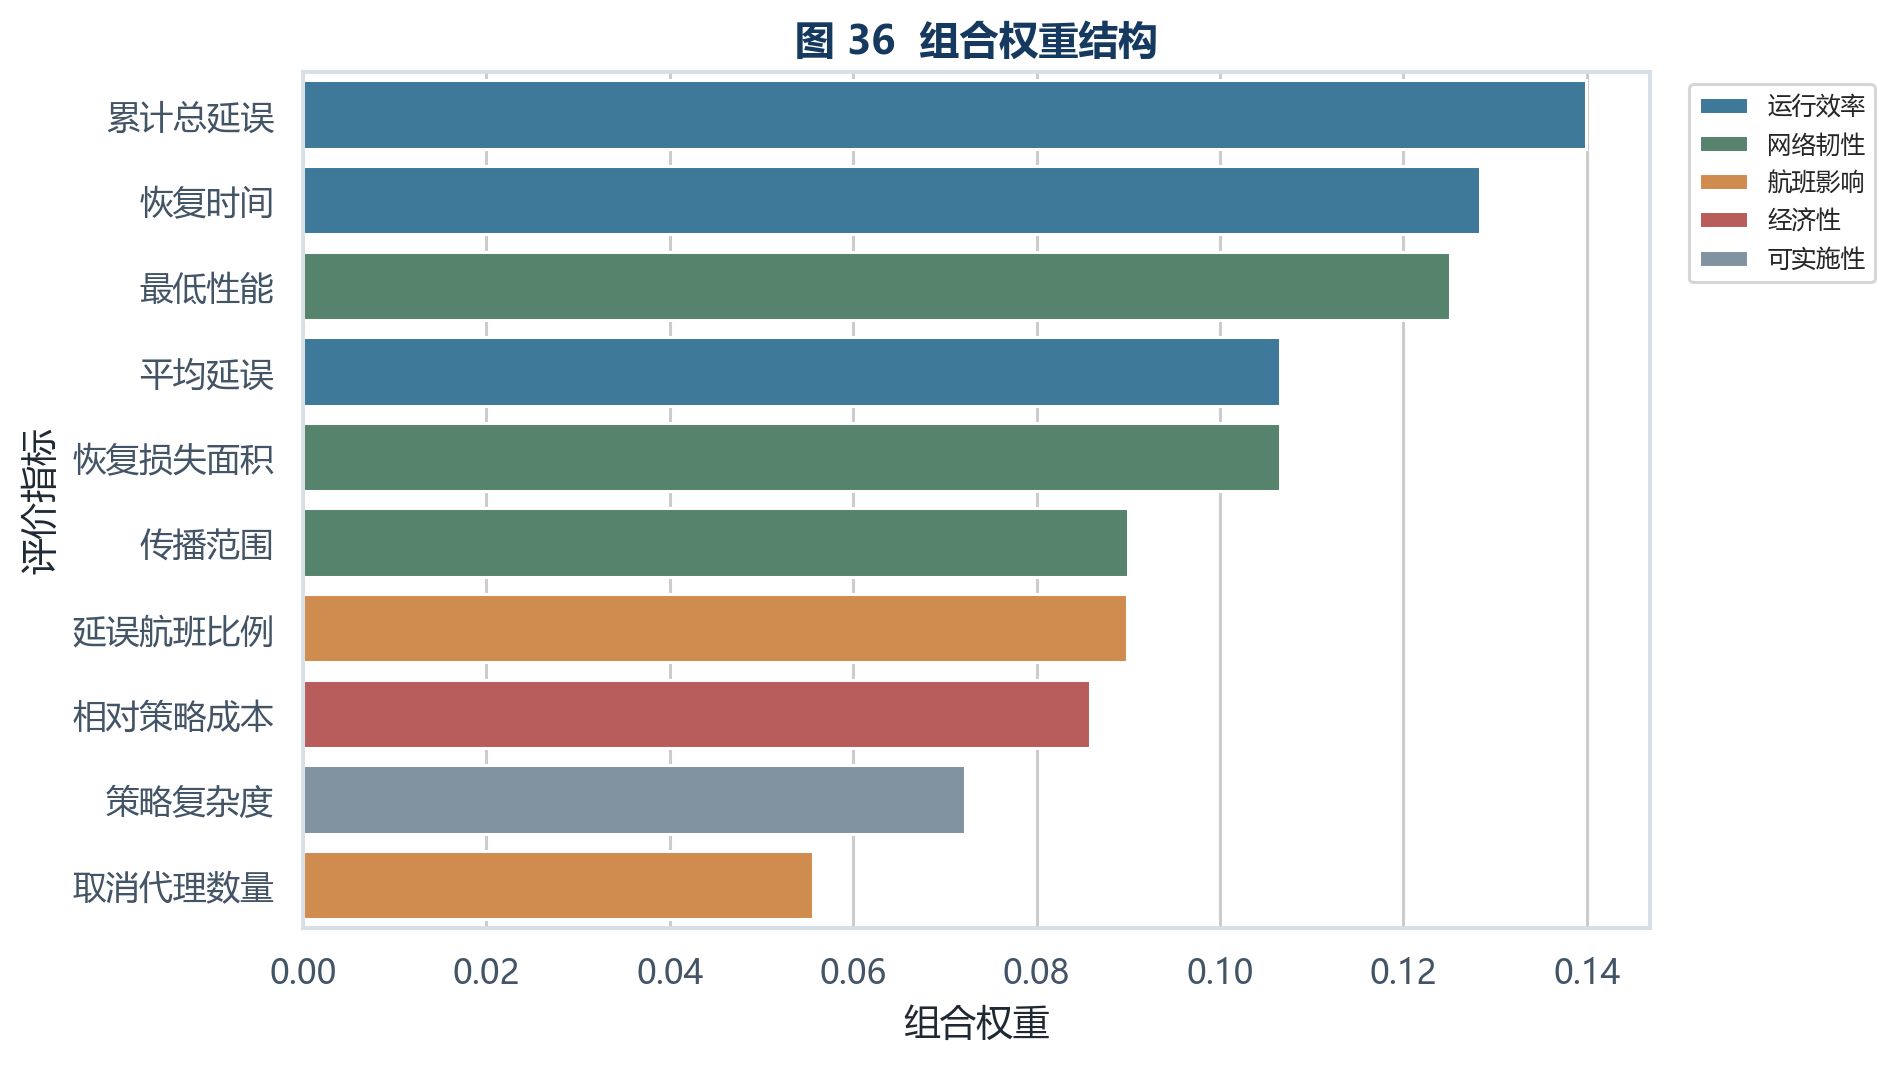
\includegraphics[width=0.86\linewidth]{../figures/fig_36_indicator_weights.png}
  \caption{组合权重结构}
  \figurenote{恢复时间、累计延误、最低性能等指标权重较高，符合本项目韧性优先的课堂决策偏好。}
\end{figure}


\begin{figure}[H]
  \centering
  
\includegraphics[width=0.86\linewidth]{../figures/fig_37_weight_sensitivity.png}
  \caption{权重敏感性与排名反转}
  \figurenote{当管理偏好更保守时，低成本策略可能反超，说明推荐需要说明适用条件。}
\end{figure}


\begin{figure}[H]
  \centering
  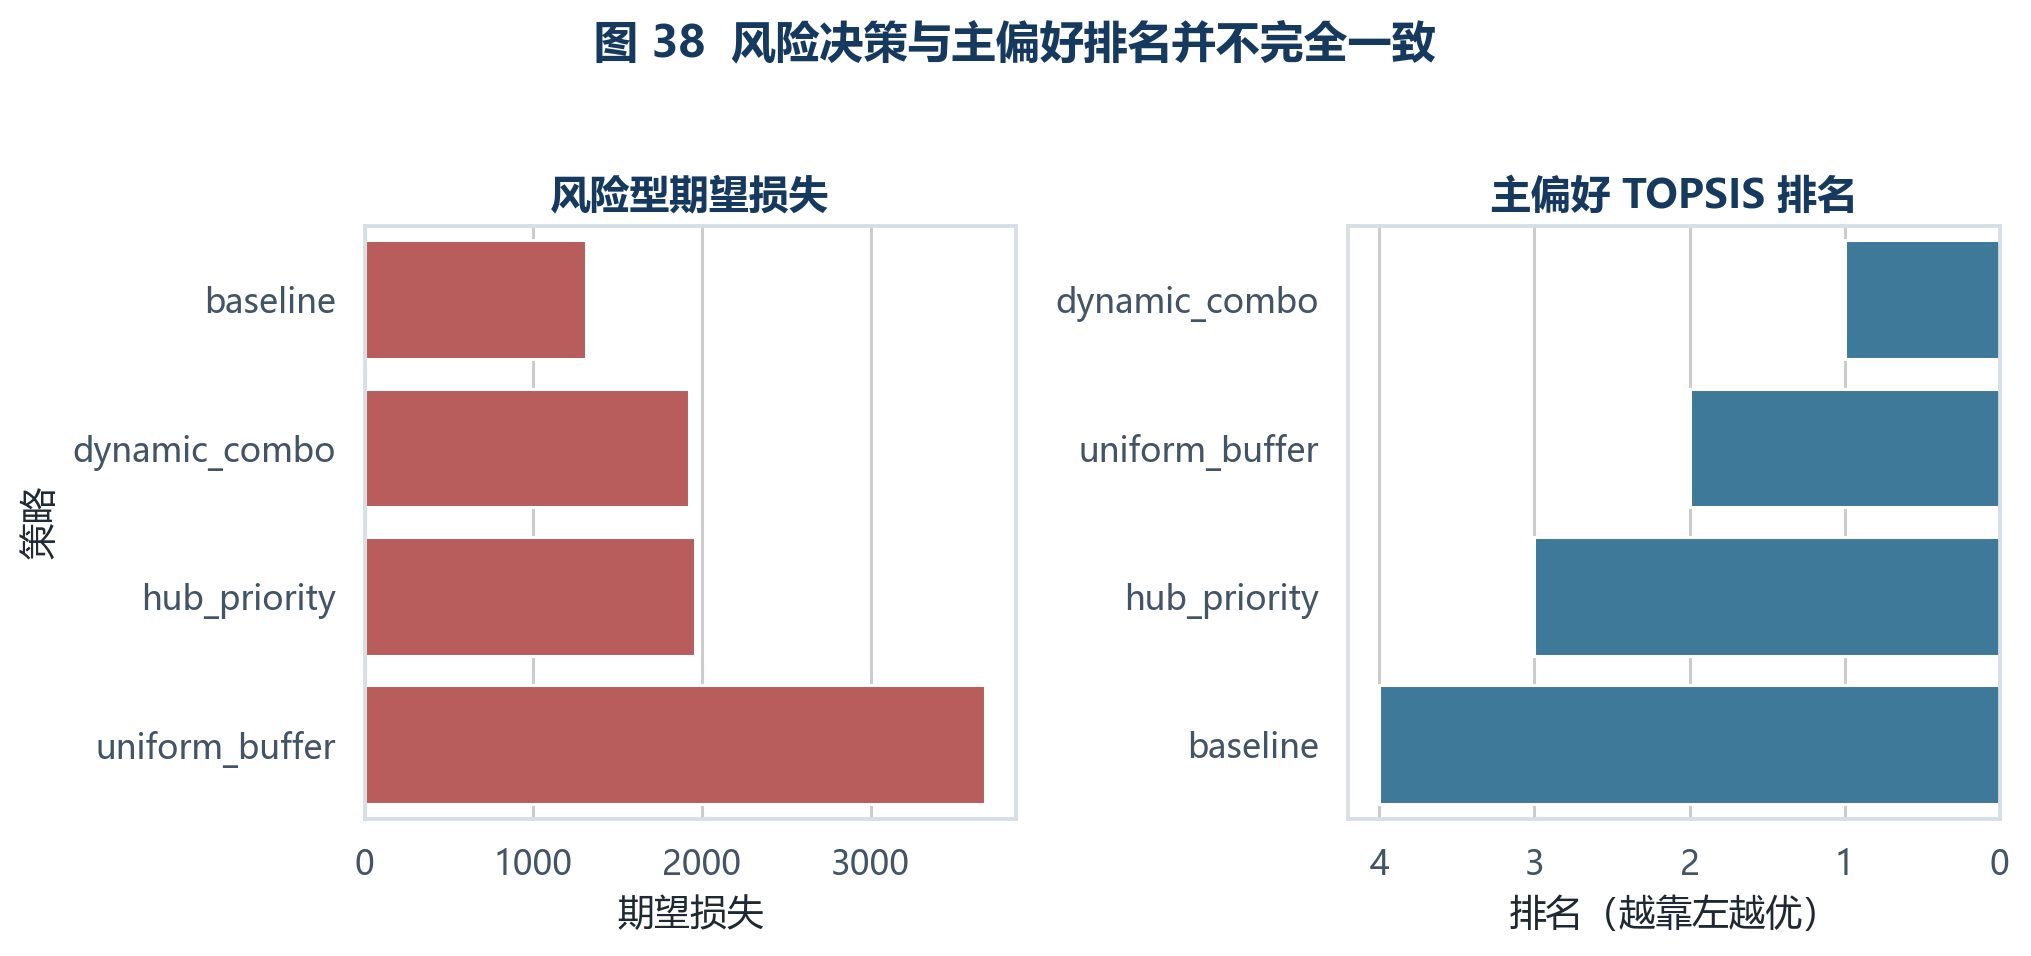
\includegraphics[width=0.86\linewidth]{../figures/fig_38_risk_vs_topsis.png}
  \caption{风险型决策与 TOPSIS 排名对照}
  \figurenote{风险准则偏向低损失、低成本，主偏好 TOPSIS 偏向恢复绩效；两者差异构成结论边界。}
\end{figure}


\section{静态 Web Demo 与部署}
静态 Web Demo 使用预计算 JSON 和浏览器端绘图，已经通过 GitHub Pages 发布。它不是单纯展示页，而是把“数据规律--预测输入--网络关键性--扰动仿真--综合决策”串成现场可检查的路径。


\begin{figure}[H]
  \centering
  
\includegraphics[width=0.82\linewidth]{../screenshots/static_web_desktop.png}
  \caption{静态 Web 首屏桌面视图}
  \figurenote{首屏展示样本范围、航班量、节点数和主推荐，避免做成空泛介绍页。}
\end{figure}


\begin{figure}[H]
  \centering
  
\includegraphics[width=0.74\linewidth]{../screenshots/static_web_fullpage.png}
  \caption{静态 Web 全页证据链}
  \figurenote{全页截图表明 Demo 覆盖从数据到决策的完整链路。}
\end{figure}


\section{结论、边界与个人体会}
第一，航空延误在本项目中更适合被理解为网络恢复问题，而不是单航班预测问题。预测模型给出风险输入，网络模型给出传播位置，状态方程给出演化过程，多准则评价给出有边界的方案建议。

第二，扩展到 30 个机场后，关键机场排序和默认冲击节点发生变化，说明结论不是固定的机场标签，而是数据范围、网络结构和风险暴露共同决定的结果。MIA、DEN、DFW、FLL、MCO 等节点在当前样本中更值得关注。

第三，动态组合 在韧性优先偏好下更优，但并非无条件最优。若决策者更重视低成本、低损失和实施简单性，基准策略 可能更合理。报告和答辩中主动说明这一点，比单纯宣称“最优策略”更接近真实管理场景。

个人体会是，系统工程作业最难的地方不在于把模型堆得多，而在于让每个模型在同一条证据链上承担明确角色。数据清洗、防泄漏、统一情景参数、可复现脚本、静态部署和结论边界都不是附属工作，它们决定了研究是否能被追问、复核和演示。后续若能接入真实机场容量、机组轮转和恢复成本，当前相对情景模型可以进一步扩展为带运营约束的优化决策模型。

\end{document}
